% Intestazione
\fancyhead[L]{5 \hspace{0.2cm} Cruscotto di valutazione della qualità} % Testo a sinistra


\section{Cruscotto di valutazione della qualità}
\label{sec:Cruscotto di valutazione della qualità}

\vspace{0.5cm}

\subsection{Varianza dell'impegno orario}
\label{subsec:Varianza dell'impegno orario}

\begin{figure}[h] 
    \centering
    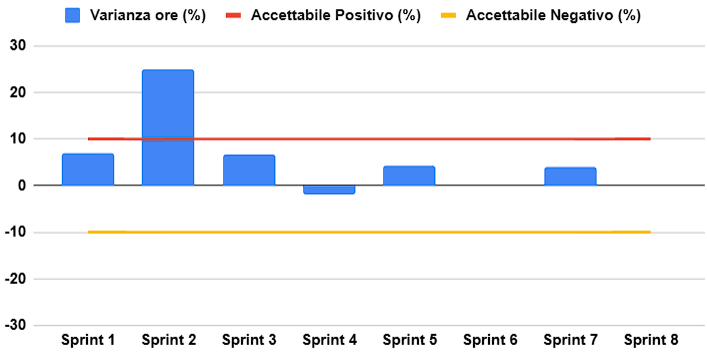
\includegraphics[width=\textwidth]{Varianza dell'impegno orario.png}
    \caption{Varianza dell'impegno orario per sprint}
    \label{fig: Varianza dell'impegno orario}
\end{figure}

\section*{Analisi}

Analizzando i valori riportati nel grafico, è riscontrabile una difficoltà nel produrre
preventivi orari vicini al consuntivato. Questo è dovuto alla scarsa esperienza del team
nel preventivare il tempo necessario per lo svolgimento delle attività. Questo problema
è stato riscontrato soprattutto nella seconda sprint, dove il team ha avuto difficoltà
nel modellare i Diagrammi dei \emph{Casi d'uso}\textsubscript{\textbf{\textit{G}}} e nel redigere i corrispettivi requisiti.
Con il progredire delle sprint, il team ha acquisito maggiore esperienza nel preventivare
il tempo necessario per lo svolgimento delle attività, riuscendo ad ottenere un valore
basso di varianza nello quarta e ultima sprint della \emph{RTB}\textsubscript{\textbf{\textit{G}}}.

\newpage

\subsection{Varianza di budget}
\label{subsec:Varianza di budget}

\begin{figure}[h] 
    \centering
    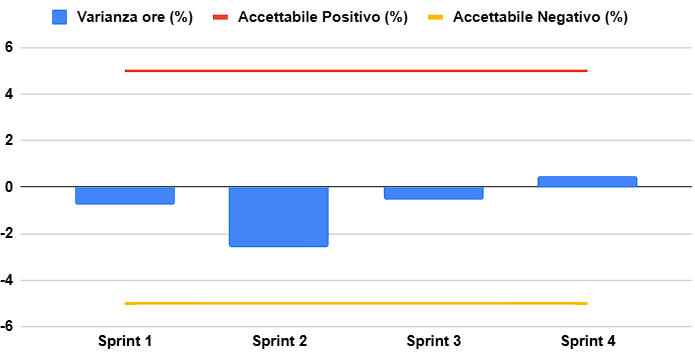
\includegraphics[width=\textwidth]{Varianza di budget.png}
    \caption{Varianza di budget per sprint} 
    \label{fig: Varianza di budget}
\end{figure}

\section*{Analisi}

Dall’analisi del grafico è immediato osservare che i valori di varianza di budget sono
sempre rimasti all’interno della soglia di accettabilità. Il risultato evidenziato è 
tuttavia migliorabile: negli sprint 1, 2 e 3 la varianza di budget è risultata negativa,
indicando che il costo effettivo è stato maggiore rispetto a quanto preventivato. In
particolare ciò si può notare in grande misura per la sprint 2, dove il team ha avuto difficoltà nel
modellare i Diagrammi dei Casi d'uso e nel redigere i corrispettivi requisiti.

\newpage

\subsection{Estimate to Complete ed Estimate at Completion}
\label{subsec:Estimate to Complete ed Estimate at Completion}

\begin{figure}[h] 
    \centering
    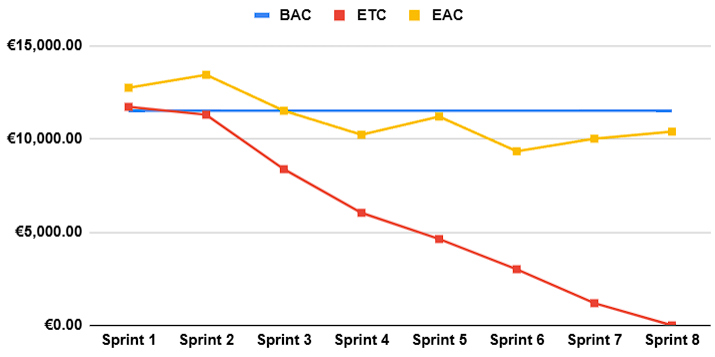
\includegraphics[width=\textwidth]{Estimate to Complete ed Estimate at Completion.png}
    \caption{Progressione Estimate to Complete e Estimate at Completion in relazione al Budget at Completion} 
    \label{fig: Estimate to Complete ed Estimate at Completion}
\end{figure}

\section*{Analisi}

Dall’analisi del grafico è immediato osservare che i valori sono andati a migliorare
nel corso delle sprint. In particolare, l’Estimate at Completion dopo la quarta sprint
è addirittura migliore del preventivo dei costi di candidatura iniziale. Per il suddetto
contrattempo dei casi d'uso, anche in questo grafico si evidenzia l'aumento dei costi tra la prima
e la seconda sprint, per poi stabilizzarsi e migliorare nel corso delle sprint successive.

\newpage

\subsection{Planned Value, Earned Value e Actual Cost}
\label{subsec:Planned Value, Earned Value e Actual Cost}

\begin{figure}[h] 
    \centering
    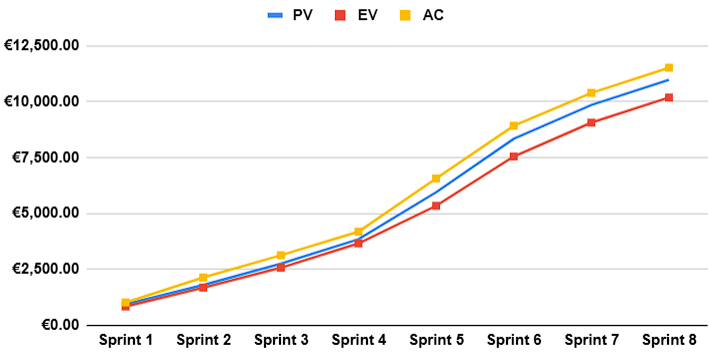
\includegraphics[width=\textwidth]{Planned Value, Earned Value e Actual Cost.png}
    \caption{Progressione Planned Value, Earned Value e Actual Cost} 
    \label{fig: Planned Value, Earned Value e Actual Cost}
\end{figure}

\section*{Analisi}

Analizzando il grafico, si può notare come i tre valori abbiano sempre progredito seguendo una
proporzione costante. In particolare, l’Actual Cost è sempre stato superiore al Planned Value,
il quale a sua volta è stato sempre superiore all’Earned Value. Questo è dovuto al fatto che
il team ha impiegato più tempo del previsto per lo svolgimento delle attività preventivate. 
Tuttavia, nella quarta sprint si evidenzia come il team
abbia migliorato la propria gestione del tempo, riuscendo a ridurre la distanza tra il Planned Value
ed l'Earned Value.

\newpage

\subsection{Schedule Variance e Cost Variance}
\label{subsec:Schedule Variance e Cost Variance}

\begin{figure}[h] 
    \centering
    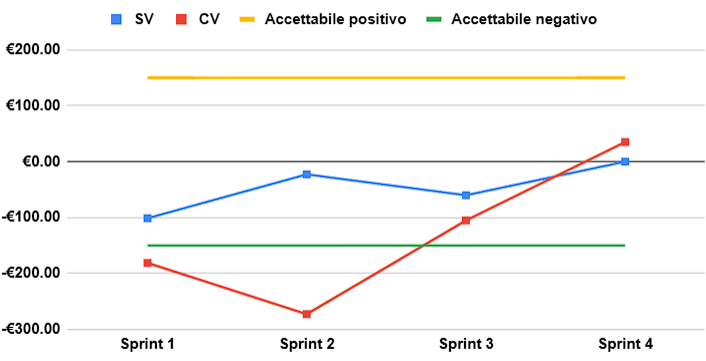
\includegraphics[width=\textwidth]{Schedule Variance e Cost Variance.png}
    \caption{Progressione Schedule Variance e Cost Variance} 
    \label{fig: Schedule Variance e Cost Variance}
\end{figure}

\section*{Analisi}

Dal grafico, risulta ancora una volta evidente come il team abbia avuto difficoltà nel
rispettare i tempi preventivati. La Schedule Variance e la Cost Variance sono infatti
risultate sempre negative, tranne nell'ultima sprint, nella quale c'è stato un miglioramento
significativo. Il risultato peggiore si registra appunto nella seconda sprint per i suddetti
motivi, che hanno comportato la discesa sotto la soglia di accettabilità per il valore della
Cost Variance, la quale tuttavia è stata migliorata nel corso delle sprint successive.

\newpage

\subsection{Schedule Performance Index e Cost Performance Index}
\label{subsec:Schedule Performance Index e Cost Performance Index}

\begin{figure}[h] 
    \centering
    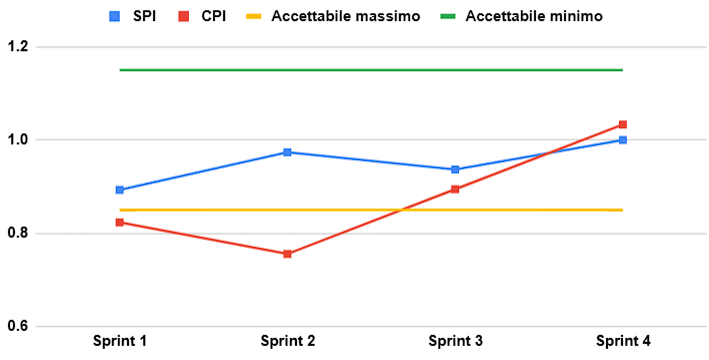
\includegraphics[width=\textwidth]{Schedule Performance Index e Cost Performance Index.png}
    \caption{Progressione Schedule Performance Index e Cost Performance Index} 
    \label{fig: Schedule Performance Index e Cost Performance Index}
\end{figure}

\section*{Analisi}

Similmente a quanto riscontrabile dall’analisi dei valori di Schedule e Cost Variance,
il valore del Cost Performance Index è sceso sotto la soglia accettabile nella 
sprint 2, per poi recuperare nelle sprint successive. Nella quarta sprint, il team
ha addirittura raggiunto un valore di Cost Performance Index superiore a 1, indicando
che il team ha speso meno risorse rispetto a quanto preventivato per lo svolgimento delle
attività. Il valore dello Schedule Performance Index è invece sempre stato inferiore a 1,
tranne nell'ultima sprint in cui è risultato pari a 0, indicando che il team ha svolto
con successo tutte le attività preventivate.

\newpage

\subsection{Misure di mitigazione insufficienti}
\label{subsec:Misure di mitigazione insufficienti}

\begin{figure}[h] 
    \centering
    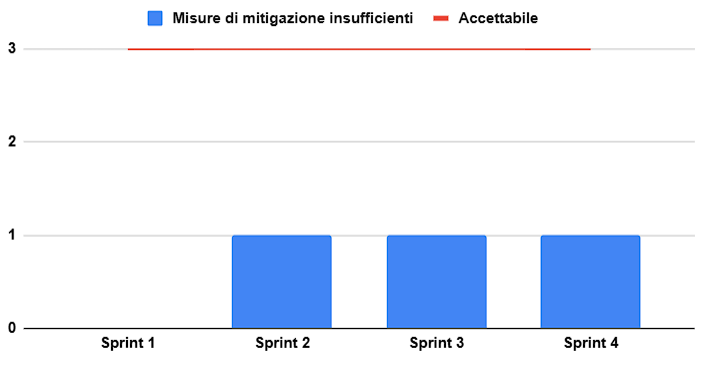
\includegraphics[width=\textwidth]{Misure di mitigazione insufficienti.png}
    \caption{Progressione occorrenza di rischi con misure mitigative insufficienti} 
    \label{fig: Misure di mitigazione insufficienti}
\end{figure}

\section*{Analisi}

Durante la RTB, il team ha riscontrato difficoltà nell'applicare alcune misure di mitigazione
per i rischi individuati. In particolare, il team ha avuto difficoltà nel gestire i rischi
legati alla comunicazione interna nella seconda sprint, dove tutti i membri hanno 
dovuto mettersi d'accordo sia sintatticamente sia semanticamente nella modellazione dei casi d'uso.
Poi, è stata riscontrata difficoltà a gestire i rischi legati alla non conformità rispetto 
agli impegni dichiarati nella terza e quarta sprint, a causa rispettivamente della concomitanza
delle vacanze natalizie e dello studio per la sessione d'esami.

\newpage

\subsection{Rischi inattesi}
\label{subsec:Rischi inattesi}

\begin{figure}[h] 
    \centering
    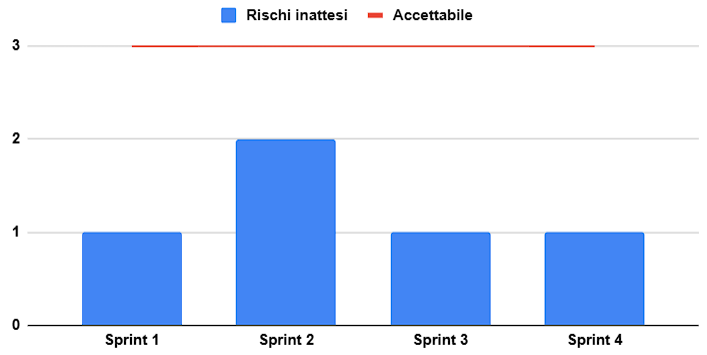
\includegraphics[width=\textwidth]{Rischi inattesi.png}
    \caption{Progressione occorrenza di rischi inattesi} 
    \label{fig: Rischi inattesi}
\end{figure}

\section*{Analisi}

Durante la RTB, il team ha riscontrato la presenza di diversi rischi inattesi. In particolare, 
il team ha incontrato rischi di confusione sulle responsabilità a causa di una spartizione di
compiti non chiara, e soprattutto rischi legati alle tecnologie: il team è stato in dubbio sulla
possibilità di utilizzare la tecnologia \emph{Docker}\textsubscript{\textbf{\textit{G}}} per la 
realizzazione del progetto in quanto non prevista inizialmente dal \emph{proponente}\textsubscript{\textbf{\textit{G}}} 
nella lista di tecnologie proposte, ma soprattutto ha avuto difficoltà nell'aiuto reciproco, poichè
la spartizione dei compiti ha previsto degli esploratori solitari per ciascuna tecnologia, rendendo poi
difficile lavorare in gruppo e chiedere aiuto ai compagni al momento dell'\emph{implementazione}\textsubscript{\textbf{\textit{G}}} del 
\emph{PoC}\textsubscript{\textbf{\textit{G}}}.

\newpage

\subsection{Requisiti soddisfatti}
\label{subsec:Requisiti soddisfatti}

\begin{figure}[h] 
    \centering
    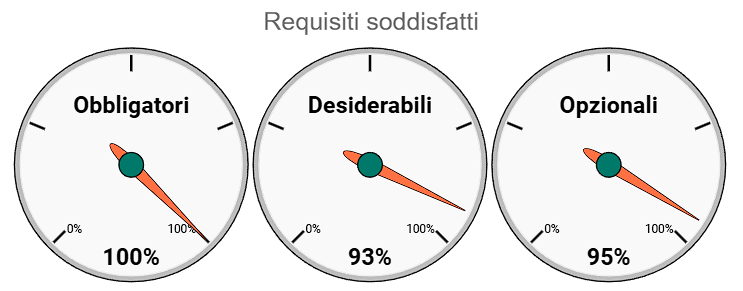
\includegraphics[width=\textwidth]{Requisiti soddisfatti.png}
    \caption{Requisiti obbligatori, desiderabili e opzionali soddisfatti} 
    \label{fig: Requisiti soddisfatti}
\end{figure}

\section*{Analisi}
Il progetto fino ad ora ha prodotto un Proof of Concept, dunque nessun prodotto finale con il quale soddisfare alcun requisito.
Per questo motivo è normale che nel cruscotto non risulti soddisfatto nessun requisito.

\newpage

\subsection{Indice di Gulpease}
\label{subsec:Indice di Gulpease}

\begin{figure}[h!] 
    \centering
    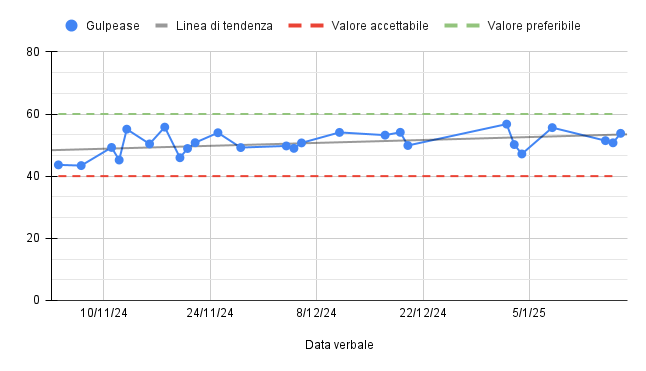
\includegraphics[width=\textwidth]{Andamento Gulpease verbali.png}
    \caption{Andamento indice di Gulpease nei verbali} 
    \label{fig: Andamento Gulpease verbali}
\end{figure}

\begin{figure}[h!]
    \centering

    \begin{minipage}{.4\textwidth}
        \centering
        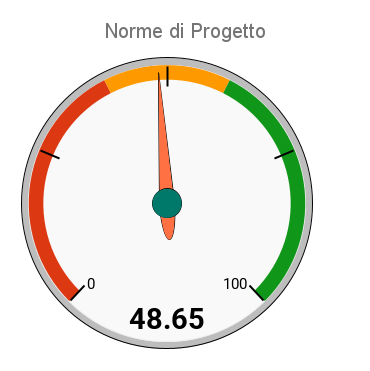
\includegraphics[width=.8\linewidth]{Gulpease Norme Progetto.png}
        \caption{}{Indice di Gulpease Norme di Progetto}
        \label{fig:Gulpease Norme Progetto}
    \end{minipage}%
    \begin{minipage}{.4\textwidth}
        \centering
        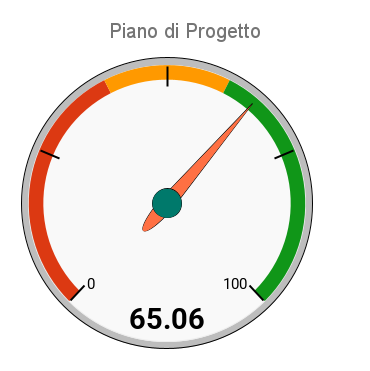
\includegraphics[width=.8\linewidth]{Gulpease Piano Progetto.png}
        \caption{}{Indice di Gulpease Piano di Progetto}
        \label{fig:Gulpease Piano Progetto}
    \end{minipage}

\end{figure}

\begin{figure}[H]
    \centering

    \begin{minipage}{.4\textwidth}
        \centering
        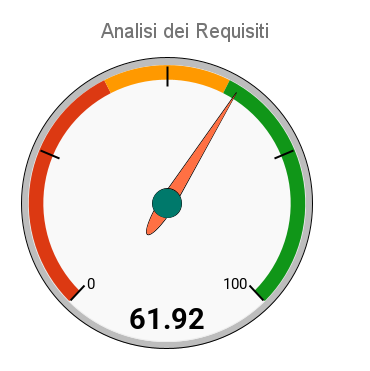
\includegraphics[width=.8\linewidth]{Gulpease Analisi Requisiti.png}
        \caption{}{Indice di Gulpease Analisi dei Requisiti}
        \label{fig:Gulpease Analisi Requisiti}
    \end{minipage}%
    \begin{minipage}{.4\textwidth}
        \centering
        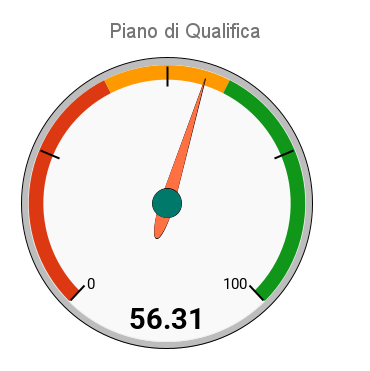
\includegraphics[width=.8\linewidth]{Gulpease Piano Qualifica.png}
        \caption{}{Indice di Gulpease Piano di Qualifica}
        \label{fig:Gulpease Piano Qualifica}
    \end{minipage}

\end{figure}

\section*{Analisi}

Questi valori mostrano che la documentazione è generalmente accessibile e comprensibile, 
dato che tutti i documenti superano la soglia accettabile di 40 nell'\emph{indice di Gulpease}\textsubscript{\textbf{\textit{G}}}, 
con la maggior parte dei valori che si avvicinano al "Valore preferibile" di 60. 
In particolare è utile notare come nel grafico relativo all'andamento dell'indice di Gulpease dei verbali la linea di tendenza sia crescente,
il che mostra un generale miglioramento da parte del gruppo nella qualità della documentazione prodotta.